\documentclass{standalone}
\usepackage{tikz}
\usetikzlibrary{shapes, positioning}

\begin{document}

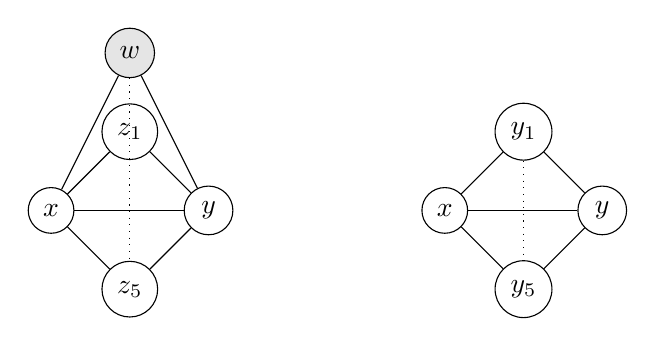
\begin{tikzpicture}

% Left diagram
\node[draw, circle] (x) at (0,0) {$x$};
\node[draw, circle] (y) at (2,0) {$y$};

\node[draw, circle, fill=black!10] (w) at (1,2) {$w$};
\node[draw, circle] (z1) at (1,1) {$z_1$};
\node[draw, circle] (z5) at (1,-1) {$z_5$};

% Connectors for left diagram
\draw (x) -- (w) -- (y);
\draw (x) -- (z1) -- (y);
\draw (x) -- (z5) -- (y);
\draw (x) -- (y);
\draw[dotted] (w) -- (z1);
\draw[dotted] (w) -- (z5);

% Right diagram
\node[draw, circle] (x2) at (5,0) {$x$};
\node[draw, circle] (y2) at (7,0) {$y$};

\node[draw, circle] (y1) at (6,1) {$y_1$};
\node[draw, circle] (y5) at (6,-1) {$y_5$};

% Connectors for right diagram
\draw (x2) -- (y1) -- (y2);
\draw (x2) -- (y5) -- (y2);
\draw (x2) -- (y2);
\draw[dotted] (y1) -- (y5);

\end{tikzpicture}

\end{document}